\chapter{Analyse paramétrique}
\section{Synthèse \texorpdfstring{\ce{NH3}}{NH3} et séparation}

Nous allons maintenant étudier de manière plus précise la dernière étape du procédé qui comprend le réacteur de synthèse d’ammoniac et l'étape de séparation des produits.
La réaction de synthèse de \ce{NH3} est suivante :
\[ \ce{N_2 + 3H2 <=> 2NH3} \]

\subsection{Manière qualitative}

Voyons de quelle manière évolue la réaction en faisant varier d'une part la température, et d'autre part la pression. Pour cela, nous nous basons sur le fait qu'une réaction chimique a toujours tendance à   aller à l'encontre des modifications qui lui sont apportées, à savoir le principe énoncé par Le Chatelier. Dans notre cas, nous devons favoriser la réaction allant dans le sens de production de \ce{NH3}.

Tout d'abord, regardons ce qu'il en est au niveau de la pression. Nous devons augmenter celle-ci car de cette manière le système réagira en favorisant le sens de réaction produisant un plus petit nombre de moles de gaz, à savoir \ce{NH3}, dans le but de rétablir la pression. 

Ensuite, nous allons étudier le comportement de notre réaction lorsqu'on modifie la température. Pour cela, nous devons déterminer si la réaction est endothermique ou exothermique. Nous calculons donc le $\Delta H$  de la réaction.
\[ \Delta H^0_r = \unit{-92,4}{\kilo\joule\per\mole} \]
Le signe de $\Delta H$ étant négatif, notre réaction est bien exothermique. De ce fait, nous devons diminuer la température afin de favoriser la réaction qui libère de la chaleur, c'est-à-dire, la réaction directe.

Nous en venons donc à la conclusion qu'il nous faudrait une pression théoriquement infinie et une température la plus basse possible. Cependant, nous sommes restreint économiquement et techniquement, nous devons donc trouver un juste milieu, une conversion totale n'est donc pas envisageable. 
\\

Une pression très élevée est économiquement et techniquement irréalisable car les tuyaux et autres équipements supportant les flux devront aligner leurs performances pour répondre à des critères beaucoup plus stricts qu'avec de basses pressions.
Pour cette raison, il serait plus judicieux de réinjecter  le diazote et le dihydrogène qui n'ont pas réagi au cours de la réaction (la réaction est à l'équilibre!) dans le réacteur. Pour effectuer cette séparation, les éléments du réacteur sont refroidis, l'ammoniac est liquéfié (l'ammoniac se condense à température plus élevé que le dihydrogène et diazote) et les réactifs sont réintroduits dans le réacteur.

\subsection{Manière quantitative}

De manière plus rigoureuse, nous pouvons démontrez l'influence de la température et de la pression sur le rendement de la réaction à l'aide d'une modélisation mathématique.

Démontrons qu'une diminution de la température favorise la production de produits pour toute réaction exothermique avec l'équation de Van't Hoff.
\[ \ln{\frac{K_2}{K_1}} = \frac{\Delta H^0_r}{R} \left(\frac{1}{T_1} - \frac{1}{T_2}\right) \]

$ \Delta H^0_r < 0$, si $T_2<T_1$ alors $1/T_2 > 1/T_1$. Donc $\ln{K_2/K_1} > 0$, ce qui implique que $K_2/K_1>1$  et donc que $ K_2>K_1$.

Si $K$ augmente, la réaction favorise les produits, le principe de Le Chatelier est donc bien vérifié pour la température.
\\

Pour la pression, il faut étudier l'influence de la pression totale $p_{tot}$ dans le quotient réactionnel $Q_r$ car $K(T)$ ne dépend que de la température. Ensuite, il suffit de comparer $Q_r$ et  $K(T)$ sans faire varier la température. 
\[ Q_r= \frac{{(\chi_\ce{NH3} p_{tot})}^2}{(\chi_\ce{N2} p_{tot}) \cdot {(\chi_\ce{H2} p_{tot})}^3}=\frac{{\chi_\ce{NH3}}^2}{\chi_\ce{N2} {\chi_\ce{H2}}^3 { (\frac{p_{tot}}{p^0}})^2} \]

Lorsque la pression augmente, $Q_r$ diminue, $Q_r < K$ et donc la réaction favorise les produits.
 
Lorsque la pression diminue, $Q_r$ augmente, $Q_r > K$ et donc la réaction favorise les réactifs.

Le principe de Le Chatelier est vérifié pour la pression.

\subsection{L’influence de la température et de la pression de
sortie du réacteur de synthèse d'ammoniac}

Pour déterminer l'influence de ces paramètres à la sortie de notre dernier réacteur, il faut établir un tableau d'avancement de notre réaction.

\begin{center}
  \begin{tabular}{lcccc}
    & $\ce{N2}$ & $\ce{3H2}$ & $\ce{2NH3}$ & $\sum$  \\
    \hline
    $n_{init}$ &
    a & b & 0 & a+b \\
    $n_{eq}$ &
    $a-\xi$ & $b-3\xi$ & $2\xi$ & $a+b-2\xi$  \\
    $\chi_i$ &
     $\frac{a-\xi}{a+b-2\xi}$ & $\frac{b-3\xi}{a+b-2\xi}$ & $\frac{2\xi}{a+b-2\xi}$ & 1 \\
     $a_i$ &
     $\chi_i \frac{p_{eq}}{p^0}$ & $\chi_i \frac{p_{eq}}{p^0}$ & $\chi_i \frac{p_{eq}}{p^0}$ & $\frac{p_{eq}}{p^0}$ \\     
  \end{tabular}
\end{center}

avec a et b respectivement le nombre de moles initiales de \ce{N2} et \ce{H2}, $\xi$ le degré d'avancement, $\chi_i$ et $a_i$ respectivement la fraction molaire et l'activité correspondante au composé $i$. 
\\

Il faut maintenant résoudre l'égalité suivante pour déterminer la variable $\xi$ et donc la quantité de \ce{NH3} (qui vaut 2$\xi$) à la sortie du réacteur en fonction de T et $p_{tot}$ : $$ Q_r = K(T) $$ 

 $$    \frac{{\chi_\ce{NH3}}^2}{\chi_\ce{N2} {\chi_\ce{H2}}^3 { (\frac{p_{tot}}{p^0}})^2} = \exp {(- \frac{\Delta G_r}{RT})}  $$
\\
\\


Notre outil de gestion(cfr. manager.Task2) nous indique que pour 1529.1 moles de \ce{N2} et 509.7 moles de \ce{H2} à T=750 K et p  = 270 bars, nous obtenons 152.2542 moles de \ce{NH3}. Ce qui correspond approximativement au rendement du procédé de Haber-Bosch (environ 15 \%).

\section{Aspen+}
Tout d'abord il est bon de dire que la première méthode nous a permis d'affiner notre modèle fait via Aspen+. L'analyse qualitative nous a permis de faire varier nos variables de manière à obtenir un meilleur rendement pour notre procédé. Cette première analyse qualitative est donc esssentielle pour assurer une bonne modélisation du procédé par Aspen+. Maintenant pour ce qui est de l'analyse qualitative il est très compliqué d'obtenir des résultats précis sans Aspen+, notamment à cause du fait que nous recyclons une partie des produits. C'est donc là que Aspen+ démontre toute son utilité en nous fournissant des valeures très précises, et ce pour chacun des flux dans notre procédé.

Les résultats de la simulation sont disponible en annexe (voir annexe \ref{Aspen}).

\begin{figure}[h]
	\begin{center}
	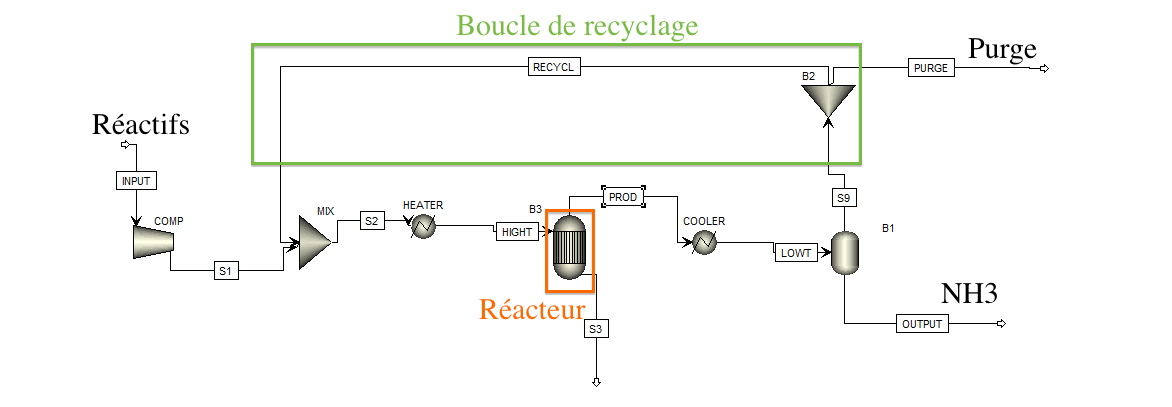
\includegraphics[scale=0.5]{task2/Simulation_final.png}
	\end{center}
	\caption{Simulation Aspen+}
\end{figure}
